% Ejercicio 12, inciso a) — issue #6. Mismo contenido que inciso-a.md.
% Fragmento sin preámbulo: lo incluye latex/main.tex, que ya pone el título del inciso.

\begin{quote}
\itshape
Identifica el patrón de diseño más adecuado, justifica tu selección basándote en las
características del problema y explica la propuesta de solución considerando las clases
que intervienen y las relaciones entre ellas. ¿Por qué no usar Strategy o polimorfismo simple?
\end{quote}

\subsubsection{Patrón seleccionado: Visitor}

Visitor representa una operación que se aplica a los elementos de una estructura de objetos,
y permite definir operaciones nuevas sin cambiar las clases de los elementos sobre los que
opera (Gamma et al., 1994, p.~366). La conferencia de la asignatura lo presenta como una forma
de separar un algoritmo de la estructura de objetos sobre la que opera, siguiendo el principio
abierto/cerrado (\emph{Marcos de Trabajo y Patrones de Diseño}, diap.~40).

En este problema, los \textbf{elementos} son las cuentas, y las \textbf{operaciones} son
visitantes: ejecutar, revertir y auditar, y las que vengan después, como «congelar cuenta» o
«calcular intereses».

\begin{quote}
El enunciado nombra tres tipos de cuenta (ahorro, corriente e inversión). El inciso~b pide
cuatro y agrega la cuenta empresarial, así que el diseño usa las cuatro.
\end{quote}

\subsubsection{Justificación}

GoF recomienda Visitor en tres situaciones (Gamma et al., 1994, p.~368), y las tres se dan en
este problema (las tres primeras filas de la tabla). Además, dos consecuencias del patrón
resuelven otros dos requisitos del enunciado (las dos últimas filas):

\begin{table}[H]
\centering
\small
\begin{tabularx}{\textwidth}{>{\raggedright\arraybackslash}X >{\raggedright\arraybackslash}X}
\toprule
\textbf{Característica del problema} & \textbf{Cómo la resuelve Visitor} \\
\midrule
\textbf{El comportamiento depende de dos cosas a la vez}: de la operación y del tipo de
cuenta. Un retiro no se ejecuta igual en una cuenta de ahorro (límite de retiros al mes), en
una corriente (sobregiro) o en una de inversión (penalización por retiro anticipado).
  & \textbf{Doble despacho}: \texttt{cuenta.Aceptar(visitante)} elige el código según la
    operación y según la cuenta, sin \texttt{if} ni \texttt{switch} por tipo (ver más
    abajo). GoF lo recomienda cuando las operaciones dependen de la clase concreta de cada
    objeto (p.~368). \\
\addlinespace
\textbf{Las operaciones no tienen relación entre sí.} Mover dinero, deshacerlo, auditar y
calcular intereses son responsabilidades distintas.
  & Cada operación queda reunida en su propia clase y no se reparte por las cuentas
    (GoF, pp.~368, 371). Por ejemplo, toda la auditoría vive en
    \texttt{AuditarTransaccion}. \\
\addlinespace
\textbf{Los tipos de cuenta son estables y las operaciones crecen.} Un banco crea productos
nuevos muy de vez en cuando; en cambio, el enunciado ya anticipa operaciones nuevas.
  & Es el caso para el que GoF recomienda Visitor: las clases de la estructura rara vez
    cambian, pero a menudo se quieren operaciones nuevas (pp.~368, 371). \\
\addlinespace
\textbf{Hay que poder añadir operaciones} («congelar cuenta», «calcular intereses»)
\textbf{sin modificar las cuentas ni las transacciones}.
  & Una operación nueva es \textbf{una clase visitante nueva}, y ninguna cuenta cambia. Según
    GoF, Visitor hace fácil añadir operaciones (p.~370). Es el principio abierto/cerrado
    aplicado a las operaciones. \\
\addlinespace
\textbf{La auditoría acumula resultados} mientras recorre las cuentas: un registro por
cuenta, y totales por sucursal en el inciso~c.
  & Un visitante puede acumular estado mientras visita los elementos (GoF, p.~372). \\
\bottomrule
\end{tabularx}
\caption{Características del problema y cómo las resuelve Visitor.}
\end{table}

\subsubsection{Propuesta de solución: clases y relaciones}

El diseño se presenta en dos figuras. La primera muestra el patrón; la segunda, las
transacciones y la auditoría. En la carpeta \texttt{diagramas} del repositorio hay una guía
para leerlas.

\begin{figure}[H]
\centering
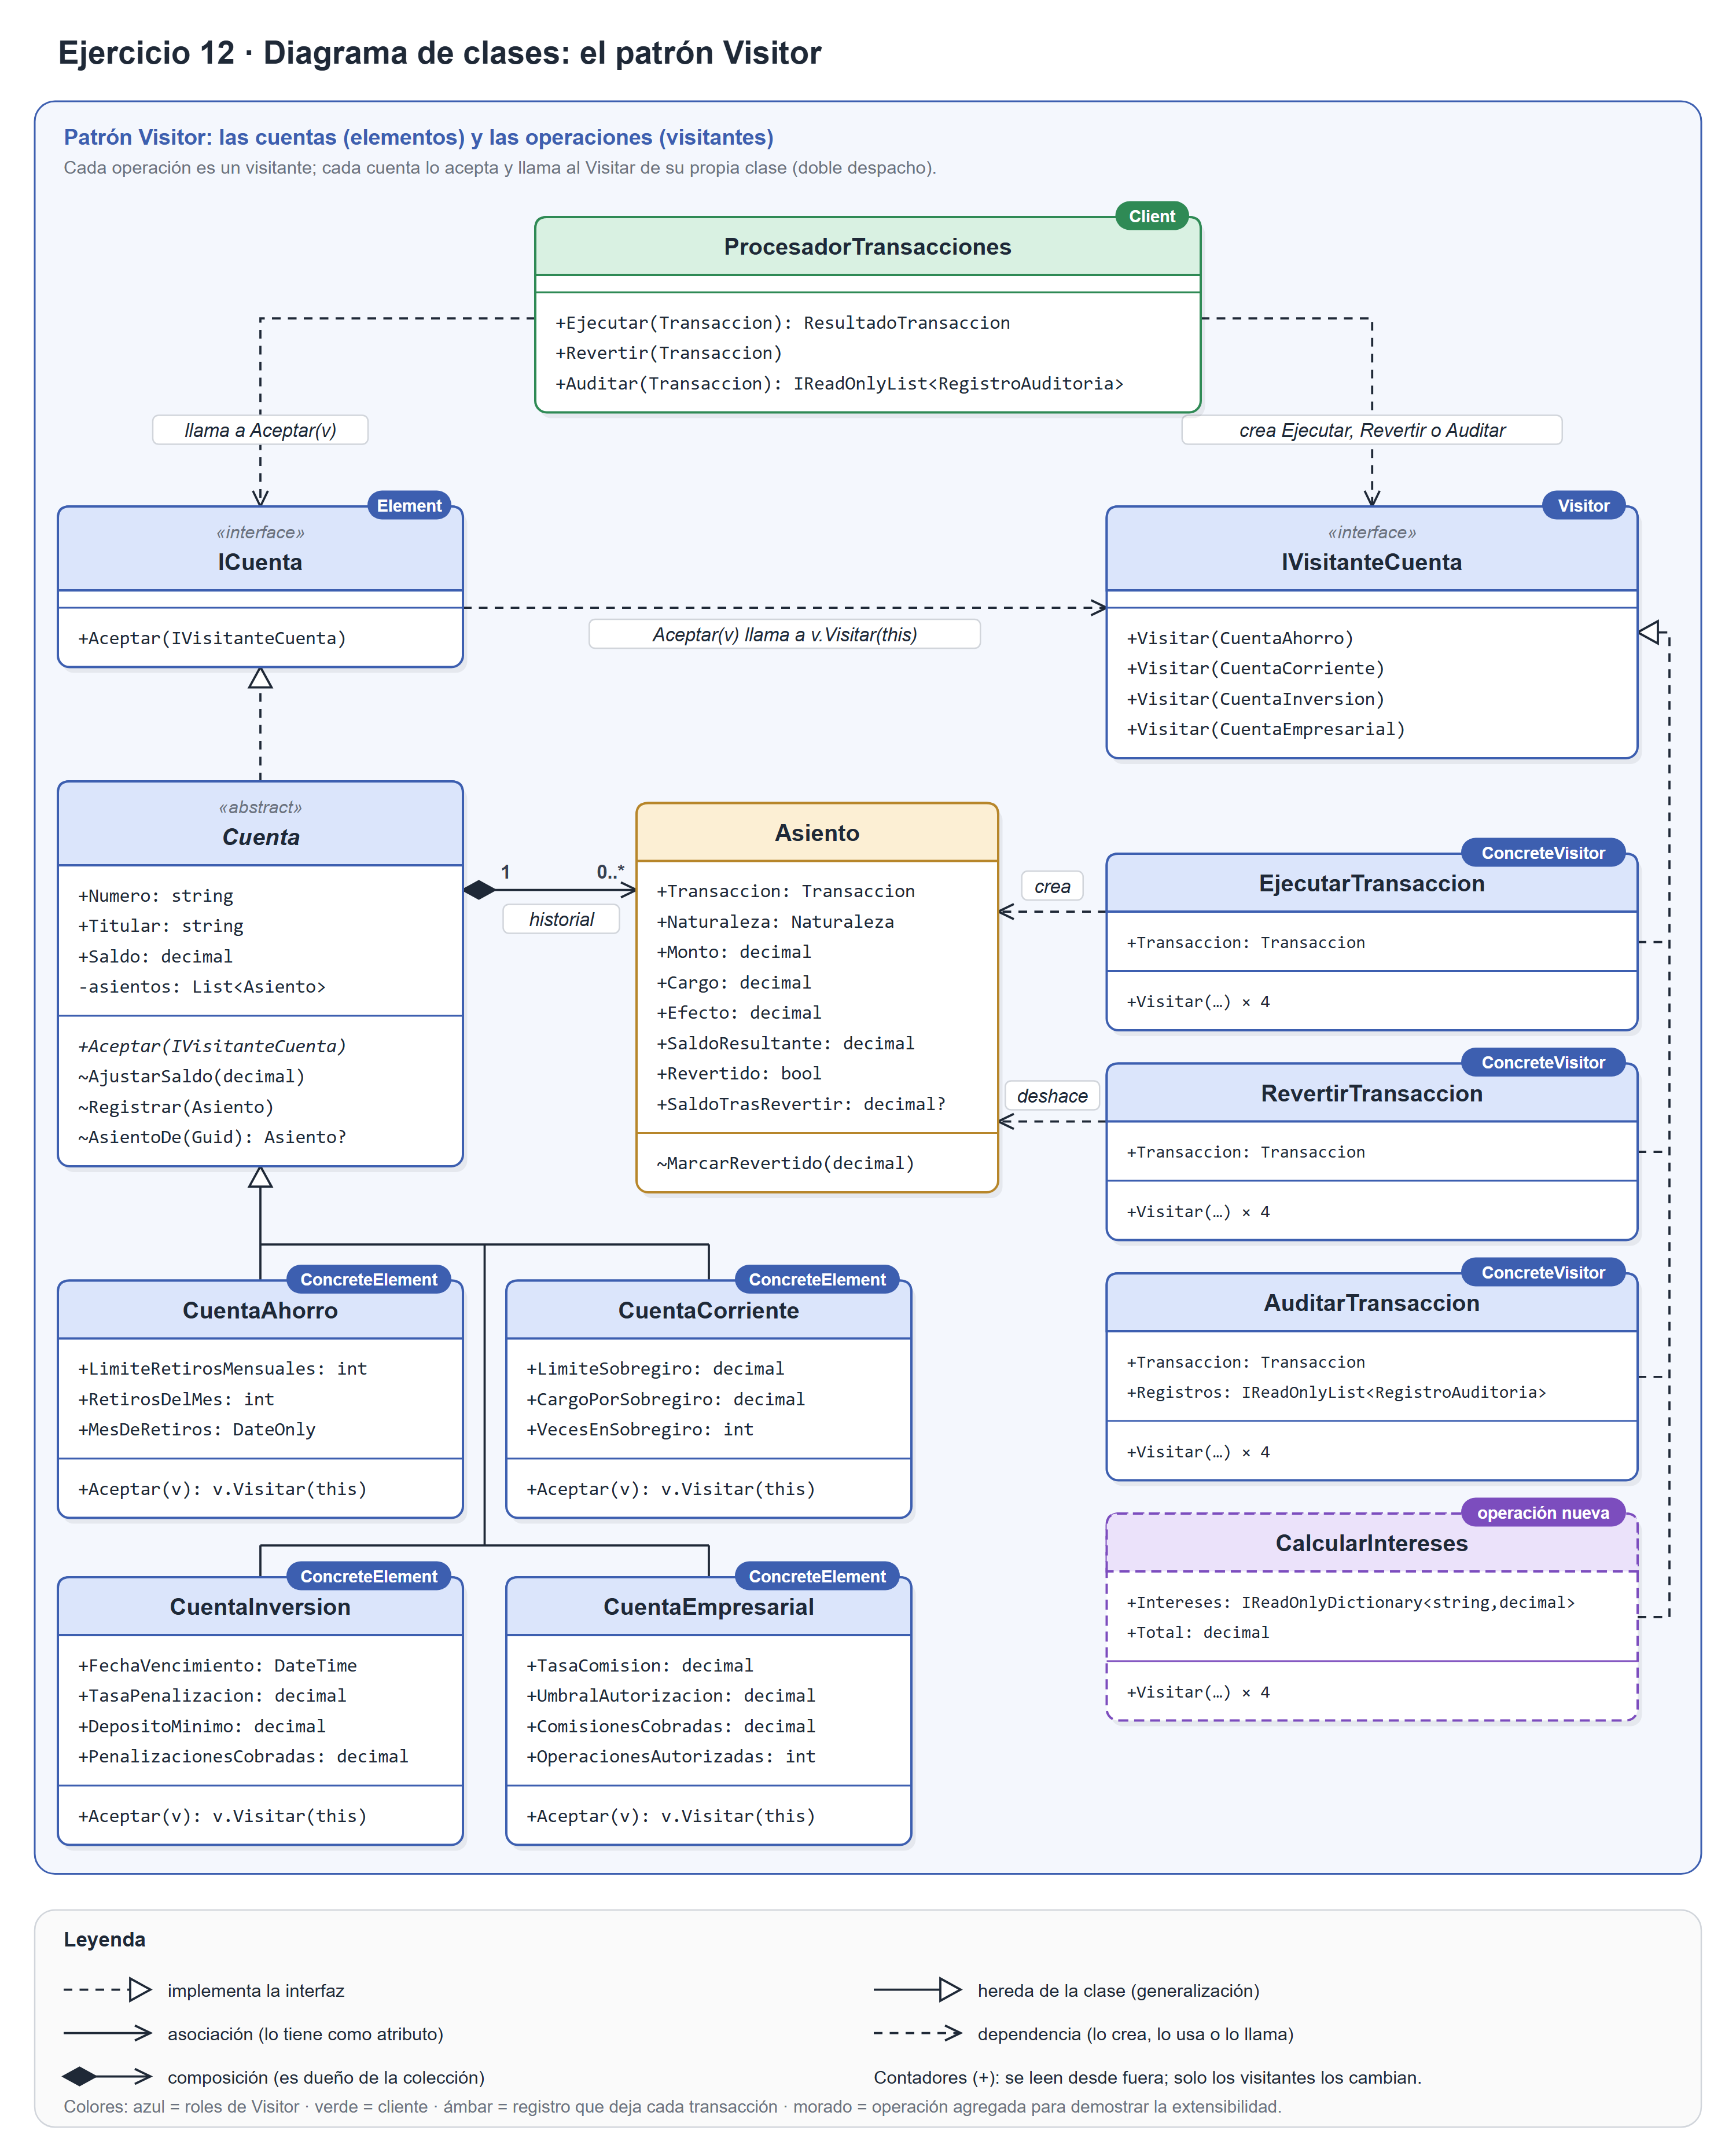
\includegraphics[width=0.95\textwidth]{ejercicio-12-transacciones-bancarias/diagramas/inciso-a-visitor.png}
\caption{Diagrama de clases, figura 1: el patrón Visitor.}
\label{fig:e12-visitor}
\end{figure}

\begin{figure}[H]
\centering
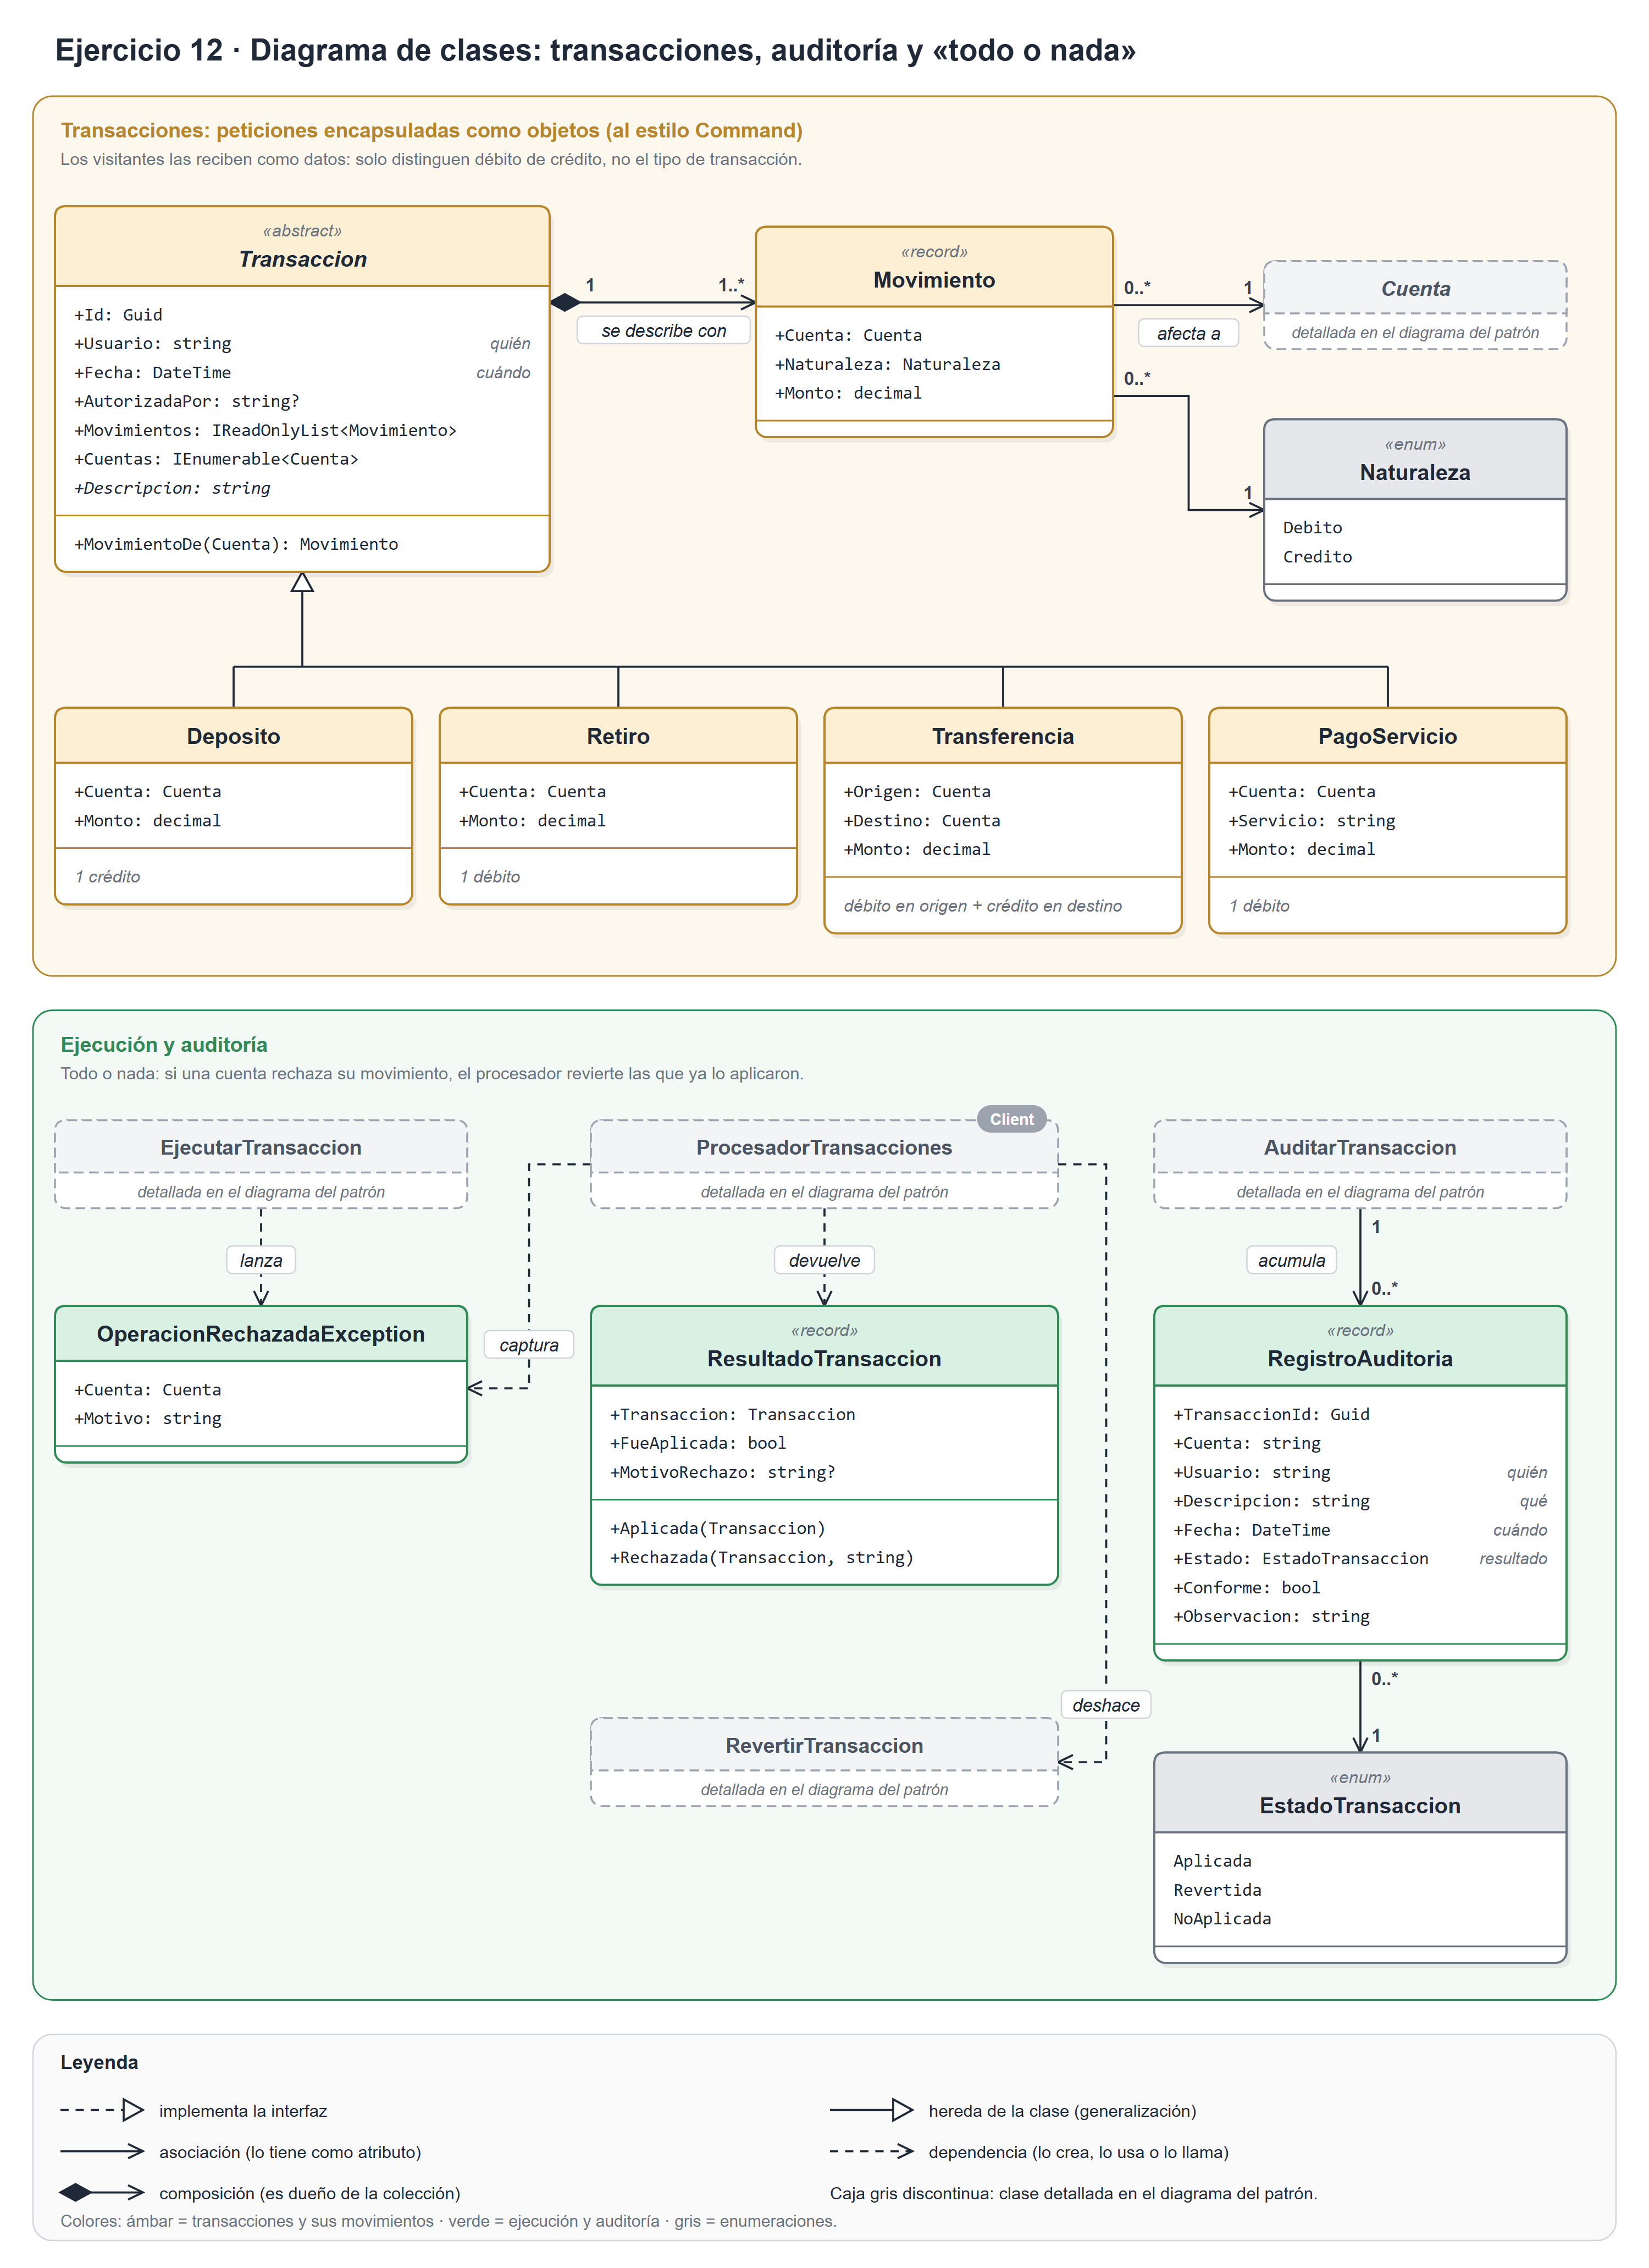
\includegraphics[width=0.95\textwidth]{ejercicio-12-transacciones-bancarias/diagramas/inciso-a-transacciones.png}
\caption{Diagrama de clases, figura 2: transacciones, auditoría y «todo o nada».}
\label{fig:e12-transacciones}
\end{figure}

\paragraph{Roles del patrón (figura~\ref{fig:e12-visitor}).}

\begin{table}[H]
\centering
\small
\begin{tabularx}{\textwidth}{>{\raggedright\arraybackslash}p{2.9cm}
                             >{\raggedright\arraybackslash}p{4.6cm}
                             >{\raggedright\arraybackslash}X}
\toprule
\textbf{Rol (GoF)} & \textbf{Clase} & \textbf{Qué hace} \\
\midrule
Element & \texttt{ICuenta}
  & Declara \texttt{Aceptar(IVisitanteCuenta)} y nada más. El inciso~c solo necesita esta
    interfaz para que un grupo de cuentas (Composite) se trate igual que una cuenta. \\
\addlinespace
ConcreteElement & \texttt{CuentaAhorro}, \texttt{CuentaCorriente}, \texttt{CuentaInversion},
                  \texttt{CuentaEmpresarial}
  & Implementan \texttt{Aceptar} con una sola línea, \texttt{visitante.Visitar(this)}, y
    guardan los parámetros y contadores de su tipo. Heredan de la clase abstracta
    \texttt{Cuenta}, que tiene lo común: número, titular, saldo e historial de asientos. \\
\addlinespace
Visitor & \texttt{IVisitanteCuenta}
  & Declara un \texttt{Visitar} por cada clase de cuenta (cuatro sobrecargas). \\
\addlinespace
ConcreteVisitor & \texttt{EjecutarTransaccion}, \texttt{RevertirTransaccion},
                  \texttt{AuditarTransaccion}
  & Las tres operaciones del enunciado. Cada \texttt{Visitar} aplica la regla de esa
    operación para ese tipo de cuenta. \texttt{CalcularIntereses} es una cuarta operación,
    agregada en el inciso~b para demostrar la extensibilidad. \\
\addlinespace
ObjectStructure & las cuentas de una transacción
  & GoF admite que sea una colección o un Composite (p.~370). Aquí son las cuentas a las que
    afectan los movimientos de la transacción; en el inciso~c será un grupo de cuentas. \\
\addlinespace
Client & \texttt{ProcesadorTransacciones}
  & Crea el visitante de la operación (\texttt{EjecutarTransaccion},
    \texttt{RevertirTransaccion} o \texttt{AuditarTransaccion}) y llama a \texttt{Aceptar} en
    cada cuenta de la transacción. Solo conoce \texttt{ICuenta}: no sabe qué tipos de cuenta
    hay ni cuáles son sus reglas. \\
\bottomrule
\end{tabularx}
\caption{Roles de Visitor en la solución.}
\end{table}

\paragraph{Relaciones y multiplicidades.}
Las cuatro cuentas heredan de \texttt{Cuenta}, que implementa \texttt{ICuenta}. Los
visitantes implementan \texttt{IVisitanteCuenta}. Cada \texttt{Cuenta} es dueña de 0 a muchos
\texttt{Asiento} (composición). Cada visitante de transacción guarda la \texttt{Transaccion}
que procesa (su atributo \texttt{Transaccion}). En la figura~\ref{fig:e12-transacciones}, cada
\texttt{Transaccion} se describe con 1 o más \texttt{Movimiento}, y cada movimiento afecta a 1
\texttt{Cuenta}.

\paragraph{El doble despacho, sin \texttt{if} ni \texttt{switch}.}

\begin{lstlisting}[basicstyle=\ttfamily\footnotesize, columns=fullflexible, keepspaces=true]
// En cada cuenta concreta (aquí, la corriente):
public override void Aceptar(IVisitanteCuenta visitante) => visitante.Visitar(this);

// En el cliente, que solo conoce ICuenta y el visitante:
cuenta.Aceptar(new EjecutarTransaccion(retiro));
\end{lstlisting}

\begin{enumerate}
  \item \textbf{Primer despacho.} \texttt{cuenta.Aceptar(...)} es una llamada virtual: se
        ejecuta el \texttt{Aceptar} de la clase real de la cuenta, por ejemplo
        \texttt{CuentaCorriente}.
  \item \textbf{Segundo despacho.} Dentro de ese \texttt{Aceptar}, \texttt{this} es de tipo
        \texttt{CuentaCorriente}, así que el compilador elige la sobrecarga
        \texttt{Visitar(CuentaCorriente)}. Como \texttt{visitante.Visitar} también es una
        llamada virtual, se ejecuta la de la operación real, \texttt{EjecutarTransaccion}.
\end{enumerate}

El código que se ejecuta depende de dos tipos, el de la operación y el de la cuenta: es lo que
GoF llama doble despacho (p.~374). En ningún momento se pregunta de qué tipo es la cuenta.
Además, si se agrega un tipo de cuenta, el programa no compila hasta que todos los visitantes
tienen su \texttt{Visitar}.

\paragraph{¿Dónde están las transacciones?}
Las transacciones (depósito, retiro, transferencia y pago de servicios) son \textbf{objetos
que encapsulan una petición}, al estilo del patrón Command. GoF menciona que Command también
se conoce como \emph{Transaction} (p.~263) y que es una forma de modelar transacciones,
entendidas como un conjunto de cambios sobre los datos (p.~266). La conferencia lo describe
como encapsular una petición para poder encolarla, llevar un registro y deshacerla
(diap.~34). Son justo las tres cosas que pide el enunciado: ejecutar, auditar y revertir.

En la figura~\ref{fig:e12-transacciones}:
\begin{itemize}
  \item \textbf{\texttt{Transaccion}} (abstracta) guarda \textbf{quién} la pidió
        (\texttt{Usuario}), \textbf{cuándo} (\texttt{Fecha}), la autorización si hace falta y
        sus \textbf{movimientos}. Las cuatro transacciones del enunciado son subclases.
  \item Cada transacción se describe con \textbf{débitos y créditos} (\texttt{Movimiento}). Un
        depósito es un crédito; un retiro o un pago, un débito; una transferencia, un débito
        en el origen y un crédito en el destino.
  \item Los visitantes \textbf{reciben la transacción como datos} en su constructor, por
        ejemplo \texttt{new EjecutarTransaccion(\allowbreak{}transaccion)}, y en cada cuenta
        aplican el movimiento que le corresponde.
\end{itemize}

\textbf{Por qué no un Command completo}, con \texttt{Ejecutar()} y \texttt{Deshacer()} dentro
de cada transacción:
\begin{enumerate}
  \item \textbf{Una operación nueva obligaría a modificar todas las transacciones.}
        «Auditar» o «calcular intereses» serían métodos nuevos en las cuatro clases de
        transacción, y el enunciado prohíbe modificarlas.
  \item \textbf{Dentro de cada \texttt{Ejecutar()} habría que preguntar por el tipo de
        cuenta}, porque un retiro no se aplica igual en una cuenta de ahorro que en una
        corriente. Volverían los \texttt{if} y \texttt{switch} por tipo.
\end{enumerate}

Con este reparto, los visitantes solo distinguen \textbf{débito de crédito}, no el tipo de
transacción. Por eso un tipo de transacción nuevo, por ejemplo un pago de nómina (un débito y
varios créditos), es solo otra subclase que describe sus movimientos: no cambia ningún
visitante ni ninguna cuenta.

\paragraph{¿Qué se guarda para poder revertir?}
Cuando \texttt{EjecutarTransaccion} aplica un movimiento, deja en la cuenta un
\textbf{\texttt{Asiento}} con la transacción, si fue débito o crédito, el monto y el
\textbf{cargo} que cobró la regla de la cuenta (comisión, penalización o cargo por
sobregiro). Es decir, se guarda \textbf{el efecto exacto que se aplicó}, no una foto del
estado anterior. El asiento también anota el saldo en que la transacción dejó la cuenta, para
que la auditoría la juzgue por lo que hizo.

\texttt{RevertirTransaccion} busca ese asiento y aplica la \textbf{operación inversa}: resta
del saldo el efecto que tuvo (en un débito devuelve el monto y el cargo; en un crédito retira
el monto). Después descuenta los contadores propios de cada tipo de cuenta: el retiro del mes
en la de ahorro, el sobregiro en la corriente, la penalización en la de inversión, y la
comisión y la autorización en la empresarial. Por último, marca el asiento como revertido
para que no se deshaga dos veces.

\textbf{Se descartó Memento}, que guarda una foto del estado para restaurarla después
(Gamma et al., 1994, p.~316; conferencia, diap.~38). Restaurar una foto \textbf{borra las
transacciones que se aplicaron después} sobre la misma cuenta. Eso pasa siempre que se
revierte una transacción que no es la última, y con operaciones en paralelo (la restricción
del enunciado) es lo habitual. Por ejemplo:

\begin{table}[H]
\centering
\small
\begin{tabular}{lr}
\toprule
\textbf{Paso} & \textbf{Saldo} \\
\midrule
Saldo inicial & 1000 \\
Retiro de 100 & 900 \\
Depósito de 50 & 950 \\
Revertir el retiro restaurando la foto anterior & 1000: \textbf{se pierde el depósito} \\
Revertir el retiro aplicando la operación inversa & \textbf{1050}, correcto \\
\bottomrule
\end{tabular}
\caption{Revertir con una foto del estado frente a revertir con la operación inversa.}
\end{table}

GoF admite que un comando que se puede deshacer guarde los argumentos de la operación que
aplicó (p.~269), y eso es lo que guarda el \texttt{Asiento}. También describe mementos que
guardan solo el cambio incremental (p.~321), pero exigen deshacer en un orden predecible, y
aquí no se cumple: se puede revertir cualquier transacción, no solo la última. La conferencia
de Arquitecturas llama a esta técnica \textbf{compensación de transacciones} (diap.~58).

\paragraph{Decisiones de diseño.}
\begin{itemize}
  \item \textbf{Las reglas de negocio viven en los visitantes, no en las cuentas.} Las cuentas
        solo guardan sus datos y parámetros: límite de retiros, tope de sobregiro, tasas y
        umbral de autorización. Así cada operación nueva trae sus propias reglas sin tocar las
        cuentas.
  \item \textbf{Todo o nada.} Una transferencia afecta a dos cuentas. Si el débito ya se
        aplicó y el crédito se rechaza (por ejemplo, el destino es una cuenta de inversión y
        el monto no llega al depósito mínimo), \texttt{ProcesadorTransacciones} deshace el
        débito con el mismo \texttt{RevertirTransaccion}. Es la base de la atomicidad que pide
        la restricción.
  \item \textbf{Revertir es una compensación obligatoria.} No aplica las reglas de la cuenta:
        si se revierte un depósito que ya se gastó, el saldo puede quedar por debajo de lo que
        permite la cuenta, y \texttt{AuditarTransaccion} lo marca como no conforme. En un
        banco, una reversión (por ejemplo, la de un cheque sin fondos) no se puede rechazar
        por falta de saldo.
  \item \textbf{La auditoría juzga la transacción, no el estado actual de la cuenta.} Revisa
        lo que dice el asiento: el cargo cobrado, la autorización y el saldo en que la
        transacción (o su reversión) dejó la cuenta. Así, una transacción correcta sigue
        siendo conforme aunque después otras cambien la cuenta.
\end{itemize}

\subsubsection{¿Por qué no usar Strategy?}

Strategy define una familia de algoritmos intercambiables para \textbf{un mismo contexto}
(Gamma et al., 1994, p.~349; conferencia, diap.~39). El despacho es simple: el código que se
ejecuta depende solo de la estrategia elegida. En este problema depende de dos cosas a la
vez, y con Strategy una de las dos queda sin resolver:

\begin{itemize}
  \item \textbf{Si cada operación fuera una estrategia} (\texttt{IOperacion.Aplicar(Cuenta)}),
        dentro de cada una habría que preguntar qué tipo de cuenta llegó:
\begin{lstlisting}[basicstyle=\ttfamily\footnotesize, columns=fullflexible, keepspaces=true]
if (cuenta is CuentaAhorro ahorro) { /* límite de retiros */ }
else if (cuenta is CuentaCorriente corriente) { /* sobregiro */ }
// ... y así con cada tipo de cuenta, en cada operación
\end{lstlisting}
        Son justo los condicionales que Strategy debería eliminar (GoF, p.~352), y el
        antipatrón \emph{Spaghetti Code} («muchos if o switch») de la conferencia (diap.~45).
        Además, si se agrega un tipo de cuenta, el compilador no avisa en qué estrategias
        falta su caso: el caso nuevo se ignora en silencio o falla en ejecución. Con Visitor, el programa no compila
        hasta que cada visitante tiene su \texttt{Visitar}.
  \item \textbf{Si cada cuenta tuviera su estrategia} (las reglas de ahorro, las de
        corriente\ldots), cada operación nueva sería un método nuevo en la interfaz de la
        estrategia y en todas sus implementaciones. Es el mismo problema que el del
        polimorfismo simple (siguiente sección).
  \item \textbf{En Strategy, el cliente elige el algoritmo}, y por eso tiene que conocer las
        estrategias (GoF, p.~353). Aquí nadie elige: la regla la impone el tipo de cuenta.
\end{itemize}

Strategy sí sería adecuado para una variación de una sola dimensión, por ejemplo cambiar la
fórmula de interés de un mismo tipo de cuenta.

\subsubsection{¿Por qué no usar polimorfismo simple?}

Polimorfismo simple sería declarar un método virtual por operación en \texttt{Cuenta}
(\texttt{Ejecutar}, \texttt{Revertir} y \texttt{Auditar}) y redefinirlo en cada cuenta.

\begin{itemize}
  \item \textbf{Cada operación nueva obligaría a modificar las cuatro clases de cuenta},
        además de la clase base: «calcular intereses» tocaría 5 clases y «congelar cuenta»,
        otras 5. Es lo que el enunciado prohíbe («sin modificar las clases de las cuentas»).
        Con Visitor, cada operación es 1 clase nueva y 0 cuentas modificadas. El inciso~d
        compara las dos opciones en detalle.
  \item \textbf{Las cuentas acumularían responsabilidades sin relación entre sí}: mover
        dinero, deshacerlo, auditar, calcular intereses\ldots{} La clase de cada cuenta
        crecería con cada operación hasta convertirse en el antipatrón \emph{The Blob} (clases
        gigantes) de la conferencia (diap.~45). GoF lo describe como «contaminar» las clases
        con operaciones (p.~368).
\end{itemize}

El polimorfismo simple solo conviene en el caso contrario: cuando los tipos de cuenta cambian
a menudo y las operaciones son fijas (GoF, p.~371). No es lo que plantea el enunciado.

\subsubsection{Desventajas de Visitor y cómo se acotan}

\begin{itemize}
  \item \textbf{Agregar un tipo de cuenta es caro.} Hay que agregar un \texttt{Visitar} a
        \texttt{IVisitanteCuenta} e implementarlo en todos los visitantes (GoF, p.~371): aquí,
        en los 3 del enunciado y en \texttt{CalcularIntereses}. Se acepta porque los tipos de
        cuenta son estables; el inciso~d lo cuantifica.
  \item \textbf{Debilita la encapsulación.} Los visitantes tienen que cambiar el saldo y los
        contadores de la cuenta, así que la cuenta debe exponerlos (GoF, p.~372). Se acota con
        \texttt{internal}: los contadores tienen lectura pública, pero solo se pueden cambiar
        desde el ensamblado del banco, y fuera de él las cuentas solo se pueden leer.
  \item \textbf{Cada visitante tiene que implementar los cuatro \texttt{Visitar}}, aunque en
        una operación dos cuentas se traten igual. Se resuelve con métodos privados comunes
        dentro del visitante (por ejemplo, \texttt{Aplicar} en \texttt{EjecutarTransaccion}),
        sin copiar código.
  \item \textbf{Las sobrecargas de \texttt{Visitar} hacen menos evidente qué método se
        llama}, porque todas tienen el mismo nombre y solo cambia el tipo del parámetro. GoF
        lo presenta como una cuestión de preferencia (p.~380, nota~10); aquí se usan
        sobrecargas porque es lo habitual en C\#.
\end{itemize}

\subsubsection{Patrones relacionados}

\begin{table}[H]
\centering
\small
\begin{tabularx}{\textwidth}{>{\raggedright\arraybackslash}p{2.3cm} >{\raggedright\arraybackslash}X}
\toprule
\textbf{Patrón} & \textbf{Relación con esta solución} \\
\midrule
Command & Las transacciones son peticiones encapsuladas como objetos (ver arriba). \\
\addlinespace
Memento & Se descartó para revertir: restaurar una foto del estado borraría transacciones
          posteriores. \\
\addlinespace
Composite & En el inciso~c, un grupo de cuentas implementa \texttt{ICuenta} y su
            \texttt{Aceptar} pasa el visitante a sus hijos. GoF lo señala como un uso típico
            de Visitor (p.~380). \\
\addlinespace
Iterator & En el inciso~c, recorre las transacciones de una cuenta sin exponer su lista
           interna. \\
\bottomrule
\end{tabularx}
\caption{Patrones relacionados.}
\end{table}

\subsubsection{Usos conocidos}

\begin{itemize}
  \item \textbf{.NET:} \texttt{System.Linq.Expressions.ExpressionVisitor} recorre árboles de
        expresiones con un método \texttt{Visit\ldots} por cada tipo de nodo. Los proveedores
        de LINQ lo usan; por ejemplo, Entity Framework lo usa para traducir consultas a SQL.
  \item \textbf{La API de Roslyn (el compilador de C\#):} \texttt{CSharpSyntaxVisitor} tiene un
        \texttt{Visit\ldots} por cada tipo de nodo del árbol de sintaxis. Es el mismo ejemplo
        con el que GoF presenta el patrón: un compilador que aplica muchas operaciones a un
        árbol de sintaxis (p.~366).
\end{itemize}

\paragraph{Referencias.}
Gamma, E., Helm, R., Johnson, R., y Vlissides, J. (1994). \emph{Design patterns: Elements of
reusable object-oriented software}. Addison-Wesley. Los números de página corresponden a la
copia del libro en la bibliografía de la asignatura (\emph{Documentacion Patrones}), igual que
en el ejercicio~9.

Ingeniería de Software. \emph{Marcos de Trabajo y Patrones de Diseño} [diapositivas de la
conferencia].

Ingeniería de Software. \emph{Arquitecturas de Software} [diapositivas de la conferencia].
